\section{Introduction}
In this assignment, a serial implementation of the Conjugate Gradient Method (CGM) was provided, which required
parallelization. In order to parallelize this implementation OpenMPI and the MPI parallelization paradigm was used.

\section{Serial Analysis}
The serial implementation of the CGM was evaluated using the provided \lstinline[language=Julia]|lap2D_5pt_n1000.mtx| matrix. This matrix
was chosen as its large size allowed for obvious parallelization opportunities to be revealed. The \lstinline[language=Julia]|perf|
profiling tool was used to analyse the serial code's execution time. From the profiling results, the \lstinline[language=Julia]|mat_vec|
function was identified as the primary computational bottleneck, accounting for approximately 86.27\% of the total execution
time. Consequently, the serial fraction of the program was estimated to be 13.73\%. The testing for the serial and
parallel code were performed on the Jed Cluster with and Intel\(R\) Xeon\(R\) Platinum 8360Y CPU, running at  2.40 GHz.


These values along with Amdahl's and Gustafson's laws for strong and weak scaling were used to calculate a theoretical
upper bound on the possible speed-ups that could be achieved using parallelization. The speed-ups were calculated using
the following equations~\cite{AmdahlGustafson2023}: 
\begin{align*}
   \text{Amdahl's Law (Strong Scaling)} = \frac{1}{(1-\alpha) + \frac{\alpha}{p}} 
\end{align*}
Here $\alpha$ is the fraction of the code that can be parallelized and $p$ is the number of processors. Gustafson's
equations are as follows:
\begin{align*}
    \text{Gustafson's Law (Weak Scaling)} = (1-\alpha) + \alpha p 
\end{align*}

\begin{figure}[h!]
    \centering
    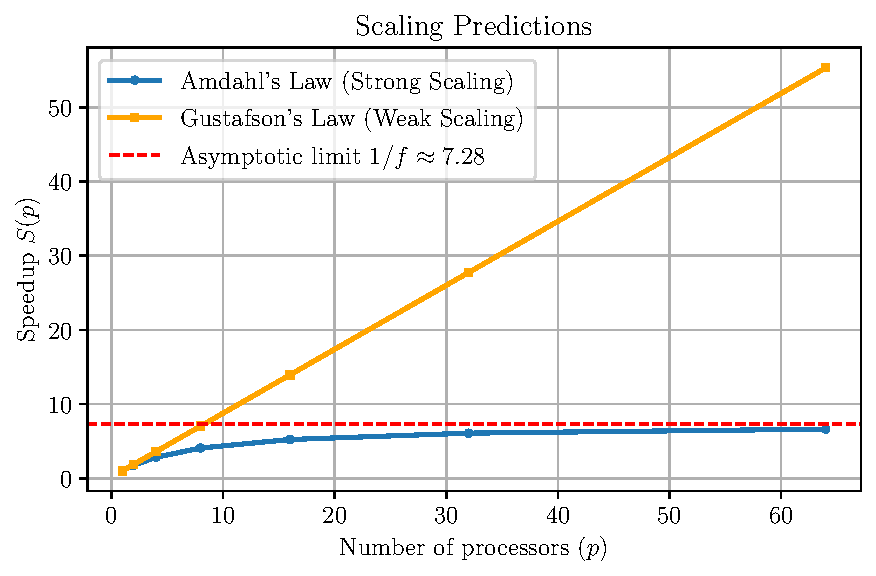
\includegraphics[width=\textwidth]{plots/scaling_laws.pdf}
    \caption{Strong and Weak Scaling Analysis using Amdahl's and Gustafson's Laws}
    \label{fig:AmdahlPlot}
\end{figure}
\FloatBarrier

\section{Parallel Modifications}
In order to parallelize the code with the least amount of communications, it was decided that the best course of action
would be to read in the matrix on processor 0 and then block distribute the row index, column index and value array to
each processor. Doing this when reading the matrix would implicitly parallelize the \lstinline[language=Julia]|mat_vec|
function and would reduce the communication needed to requiring just one \lstinline[language=Julia]|MPI_Allgather| after
each call to \lstinline[language=Julia]|mat_vec|, rather than a \lstinline[language=Julia]|MPI_Scatterv| and a
\lstinline[language=Julia]|MPI_Allgather| before and after the \lstinline[language=Julia]|mat_vec| calls. MPI message
packing and unpacking were also used to speed up this initial data transfer. This was enough to show some initial
improvements over the serial execution of the code, however, there was a lot more that could be done in the
\lstinline[language=Julia]|CGSolverSparse::solve()| function to further improve the parallelization of the code. Further
optimization was achieved through the use non-blocking transfers such as \lstinline[language=Julia]|MPI_Iallgatherv| as
well as combined communications such as \lstinline[language=Julia]|MPI_Reduce_scatter|. Using these combined
communications allows the MPI compiler to perform further optimizations when compiling the code. I also made use of
cblas operations such as \lstinline[language=Julia]|cblas_dcopy|, \lstinline[language=Julia]|cblas_daxpy| and
\lstinline[language=Julia]|cblas_ddot| to make use of the optimized implementations in the cblas library.

\section{Parallel Performance}